\chapter{\label{a:interferometry}Interferometric fundamentals}
\section{Interferometer fields}
* Intro to field equations of Fabry-Perot. Perhaps generalise to Michelson? Point reader towards analytical calculation of DRFPMI (Ken Strain paper).

We define the field amplitude of light across dimension $x$ as:
\begin{equation}
  \label{eq:field-amplitude}
  E = E_0 \text{e}^{\text{i} kx},
\end{equation}
for initial amplitude $E_0$ and wavenumber $k = \frac{2 \pi}{\lambda}$, where $\lambda$ denotes wavelength. Upon transmission through an optic, the transmitted field is equal to the input field, $E_{\text{in}}$, scaled by the optic's field transmissivity, $t$:
\begin{equation}
  \label{eq:transmitted-field}
  E_{\text{t}} = tE_{\text{in}}.
\end{equation}
The reflected field is similarly scaled by the optic's field reflectivity, $r$:
\begin{equation}
  \label{eq:reflected-field}
  E_{\text{r}} = \text{i}rE_{\text{in}}.
\end{equation}
Note the presence of complex coefficient $\text{i}$, equivalent to a multiplication by $\text{e}^{\text{i} \frac{\pi}{2}}$. This shows that the phase difference between reflected and transmitted fields is $\frac{\pi}{2}$, which is required for energy conservation. We choose to apply this phase shift to the reflected field by convention (see Appendix\,\ref{a:reflection-phase}).

\section{Simple cavities}
\note{Make sure this is consistent with PDH description etc. later, i.e. reflected field is E7 or whatever, etc.}

\begin{figure}
  \centering
  \includegraphics[width=\columnwidth]{graphics/generated/from-svg/AA-fabry-perot.pdf}
  \caption{\label{fig:fabry-perot}\FP{} cavity with its mirror input and output coefficients. Coefficients $a_1$ and $a_5$ are for the fields incident upon the cavity from either side, whilst $a_4$ and $a_8$ are for the fields leaving the cavity on either side. Coefficients at the outputs of the \FP{} can be calculated from inputs $a_1$ and $a_5$. The mirrors in the cavity are separated by free space through which the fields leaving each mirror's inside surface propagate.}
\end{figure}

Combining Equations \ref{eq:field-amplitude}, \ref{eq:transmitted-field} and \ref{eq:reflected-field} allows us to determine the field amplitude at different ports of a collection of mirrors. Combinations of mirrors produce \emph{optical cavities}, which possess the property that they can, under certain conditions, accumulate light power. If we take the simplest of examples, the two-mirror \FP{} cavity (see Figure\,\ref{fig:fabry-perot}), we can determine the fields coefficients present at the output nodes of the mirrors to be:

\begin{equation}
  \label{eq:fabry-perot-coefficients-1}
  \begin{split}
    a_1 &= it_1 a_0 + r_1 a_5, \\
    a_3 &= it_2 a_2, \\
    a_4 &= r_2 a_2, \\
    a_6 &= r_1 a_0 + it_1 a_5.
  \end{split}
\end{equation}

Similarly, the coefficients at the input nodes within the cavity can be determined from the output nodes of the opposite mirrors and the separation $D$:
\begin{equation}
  \label{eq:fabry-perot-coefficients-2}
  \begin{split}
    a_2 &= a_1 \text{e}^{\text{i} kD}, \\
    a_5 &= a_4 \text{e}^{\text{i} kD}, \\
  \end{split}
\end{equation}

Note the lack of a field input from the right side of the cavity in Figure\,\ref{fig:fabry-perot}. In general this field is present and has a small effect on the coefficients, but in gravitational wave detectors it is typically small by design. As this additional term adds mathematical complexity but not significant additional clarity, it has been neglected.

The coefficients in Equations \ref{eq:fabry-perot-coefficients-1} and \ref{eq:fabry-perot-coefficients-2} can be used to determine the field amplitude at different points of the interferometer. As there is only one input field in this example, the coefficients can be reduced to depend only on $a_0$, $r_1$ and $r_2$, $t_1$ and $t_2$ and $D$. The light reflected from the \FP{} is an important field to know as this is used in many experiments to assist with interferometer sensing and control. Coefficient $a_6$ determines the reflected field, but this depends on $a_0$ and $a_5$, the latter being one of the coefficients inside the cavity. Coefficient $a_5$ can have terms progressively substituted as follows:
\begin{equation}
  \label{eq:fabry-perot-reflected-coefficient}
  \begin{split}
    a_5 &= a_4 \text{e}^{\text{i} kD} \\
        &= a_2 r_2 \text{e}^{\text{i} kD} \\
        &= a_1 r_2 \text{e}^{\text{2i} kD} \\
        &= r_2 \left( it_1 a_0 + r_1 a_5 \right) \text{e}^{\text{2i} kD}, \\
  \end{split}
\end{equation}
where we find that the equation for $a_5$ depends on itself. This shows how the cavity operates: on each subsequent round trip, the cavity field is enhanced with addition field in the form of light transmitting through the first mirror. The field builds up until the amount of light entering the cavity is equal to the amount leaving. We can manipulate Equation\,\ref{eq:fabry-perot-reflected-coefficient} to show this:
\begin{equation}
  a_5 = a_0 \frac{it_1 r_2 \text{e}^{2ikD}}{1 - r_1 r_2 \text{e}^{2ikD}},
\end{equation}
where it is clear to see that the cavity coefficient depends on the input coefficient $a_0$. The coefficient representing the reflected light from the interferometer is then just $a_5$ scaled by $t_1$, with the addition of the light reflected before entering the cavity:
\begin{equation}
  a_6 = a_0 \left( r_1 - \frac{t_1^2 r_2 \text{e}^{2ikD}}{1 - r_1 r_2 \text{e}^{2ikD}} \right).
\end{equation}

With $a_6$ expressed in terms of $a_0$, we can then calculate the reflected field amplitude as a function of the input field. The output field as a function of input field $E_{\text{in}}$ is then simply:
\begin{equation}
  \label{eq:fabry-perot-field}
  \begin{split}
    E_{\text{out}} &= a_6 E_{\text{in}} \\
                   &= E_{\text{in}} \left( r_1 - \frac{t_1^2 r_2 \text{e}^{2ikD}}{1 - r_1 r_2 \text{e}^{2ikD}} \right) \\
                   &= E_{\text{in}} T.
  \end{split}
\end{equation}
The term in brackets in Equation\,\ref{eq:fabry-perot-field} is termed the \emph{transfer function} of the cavity, i.e. the ratio of the output field with respect to the input field. This is an important figure of merit for cavities and will be especially important in the later chapters of this work \note{change this to IS important in chapters xxx...}.

The reflected field transfer function $T$ is shown in Figure\,\ref{fig:cavity-tf}. This shows that when the cavity resonance condition is not met, the field incident upon the \gls{ITM} is mainly reflected. Close to resonance, the phase of the incident light and the \gls{ITM} is favourable for transmission, leading to the majority of the light being transmitted into the cavity. The width of the trough is determined by the cavity mirror transmissivities and reflectivities. \note{Define ITM in Figure A.1}

\begin{figure}
  \centering
  \includegraphics[width=\columnwidth]{graphics/generated/from-python/AA-cavity-tf.pdf}
  \caption{\label{fig:cavity-tf}Reflected field transfer function for a simple \FP{} cavity. When the cavity is on resonance, the reflected field drops to almost zero as the field coupling coefficients of the ITM favour transmission over reflection. Away from resonance, the coupling coefficients favour reflection over transmission. In this example the mirror reflectivities are $r_1 = r_2 = 0.99$, which is a configuration known as an \emph{impedance matched} cavity. A more complete description of the behaviour of cavities with different mirror reflectivities can be found in, for example, \cite{Freise2010}.}
\end{figure}

For asymmetric cavities, cavities with non-unity end mirror transmissivity and more complicated arrangements such as compound mirrors, the algebra involved in calculating transfer functions quickly becomes unwieldy and it is beneficial to utilise simulation tools (see Appendix\,\ref{a:simulation-tools}).

\subsection{\label{sec:cavity-fom}Cavity figures of merit}
Resonance is achieved within a \FP{} cavity by making the microscopic length equivalent to an integer number of half-wavelengths for a given carrier. For this we can look at the ratio of the field in the cavity to the field entering it:
\begin{equation}
  \frac{a_1}{a_0} = \frac{\text{i} t}{1 - r_1 r_2 \text{e}^{2\text{i}kD}},
\end{equation}
but we see that the denominator contains a complex exponential with maxima in both the sine and cosine quadratures. In reality, we measure the light power with photodetectors, so taking the square of the modulus leads to:
\begin{equation}
  \begin{split}
    \left|\frac{a_1}{a_0}\right|^2 &= \frac{t^2}{1-r_1 r_2 \text{e}^{2\text{i}kD} - r_1 r_2 \text{e}^{-2\text{i}kD} + r_1^2 r_2^2} \\
                                   &= \frac{t^2}{1 - 2 r_1 r_2 \cos{\left( 2kD \right)} + r_1^2 r_2^2},
  \end{split}
\end{equation}
which occurs when $kD$ becomes an integer multiple of $\pi$. This means that either the wave number, representing carrier wavelength, or the cavity length can be controlled to achieve cavity resonance. Both of these techniques are used in interferometry, sometimes simultaneously. The wavelength of a laser can usually be trimmed via a piezoelectric transducer or a heating element on the laser crystal. This results in a different output wavelength, which changes the number of wavelengths that can fit inside the cavity length and therefore can be used to achieve resonance for a particular length. The cavity length can be controlled with actuators on the mirrors: typically voice coils and magnets, these have also been implemented in the form of piezoelectric transducers and more exotic devices such as electrostatic drives.

As the resonance condition requires only an integer multiple of $\pi$, it is clear to see that resonance within the cavity is periodic as a function of laser frequency or length. A plot of the resonance condition as a function of length and frequency is shown in Figure\,\ref{fig:cavity-fsr}. The resonant peaks occur for every half wavelength offset from the nominal length (\SI{10}{\meter}). Conversely, the resonant peaks also occur in terms of frequency offsets from the nominal carrier frequency ($f = \frac{c_0}{\lambda}$). For this cavity, the frequency offset between resonant peaks is approximately \SI{15}{\mega\hertz}. For a much longer cavity, such as that of Advanced LIGO\textemdash \SI{4}{\kilo\meter}\textemdash the frequency offset reduces to approximately \SI{37.5}{\kilo\hertz}. The difference arises from the fact that a change in laser frequency will change the wavelength, and a longer cavity can fit more waves, so a smaller frequency offset is required for the same change in effective length.

\begin{figure}
  \centering
  \includegraphics[width=\columnwidth]{graphics/generated/from-python/AA-cavity-fsr.pdf}
  \caption{\label{fig:cavity-fsr}Resonant enhancement of input light in a cavity. When the length offset from zero is an integer number of half-wavelengths, the cavity enhances the input power many times over. When the offset is between integer half-wavelengths, it is anti-resonant and the cavity power is much smaller than the input power. In this example, the mirror properties are $r_1 = 0.99$, $r_2 = 1$, $t = \sqrt{1 - r_1^2}$ and the cavity's macroscopic length is \SI{10}{\meter}.}
\end{figure}

The frequency offset between successive resonant peaks is termed the \emph{free spectral range} (\gls{FSR}). This figure of merit provides some idea of the bandwidth a control system may need to be able to hold a cavity resonant.

Another figure of merit for a \FP{} cavity is the \emph{full-width at half-maximum} (\gls{FWHM}), or \emph{linewidth}, which represents the width of a resonant peak at half of its maximum power, in units of frequency. As the width of the resonant peak is a function of mirror reflectivity, the \gls{FWHM} is defined:
\begin{equation}
  \text{FWHM} = \frac{c_0}{\pi L} \sin^{-1}{\left( \frac{1 - r_1 r_2}{2 \sqrt{r_1 r_2}} \right)}.
\end{equation}

The ratio of the \gls{FSR} to the \gls{FWHM} defines the cavity \emph{finesse}, $\mathcal{F}$, defined as:
\begin{equation}
  \mathcal{F} = \frac{\text{FSR}}{\text{FWHM}} = \frac{\pi}{2 \sin^{-1}{\frac{1 - r_1 r_2}{2 \sqrt{r_1 r_2}}}},
\end{equation}
which indicates the cavity's ability to store photons. It is closely related to the quality factor $Q$, namely the ratio of the energy stored in the cavity to the energy lost per radian of oscillation, via the relation \cite{Band2006}:
\begin{equation}
Q = \frac{f_0}{\text{FSR}} \mathcal{F}.
\end{equation}
The finesse and quality factor indicate the time it would take for light to escape a resonant cavity in the event that the input light source were to be removed. A more technical use for the finesse figure is to quickly approximate the stored power in a cavity on resonance as a function of the input. \note{Show example of high and low finesse plots}

\section{\label{sec:signal-sidebands}Signal sidebands}
The field due to motion of a mirror $\Delta x$ at a distance $x$ can be determined by combining Equations \ref{eq:field-amplitude} and \ref{eq:reflected-field}. As the light must travel distance $2x$ to get to and from the optic, the field picks up a factor of $\text{e}^{2\text{i}k \left( x + \Delta x \right)}$ in phase and a factor of $r$ in amplitude:
\begin{equation}
  E_{\text{r}} \left( x \right) = r E_0 \text{e}^{2\text{i} k \left( x + \Delta x \right)}.
\end{equation}
For clarity, we can express the constant $x$ term as a static phase representing the carrier, separated from $\Delta x$ via the wave number:
\begin{equation}
  \label{eq:field-amplitude-phase}
  E_{\text{r}} \left( t \right) = r E_0 \text{e}^{\text{i} \left( 2 \omega_0 t + k \Delta x\right)}.
\end{equation}
It is possible to express any particular motion in the form of a series of sinusoidal functions. Expressing mirror motion as a single frequency sinusoid modulating the impinging field, we see:
\begin{equation}
  \label{eq:field-phase-modulation}
  E_{\text{r}} \left( t \right) = E_0 \text{e}^{\text{i} \left(\omega_0 t + m \cos{\left( \omega t \right)} \right)},
\end{equation}
where we introduce $m$ as the \emph{modulation depth}, a dimensionless number expressing the strength of the mirror motion. Note that we have neglected for now the reflection term $r$. With some algebraic manipulation involving Bessel functions, we can express this as \cite{Freise2010}:
\begin{equation}
  \label{eq:field-phase-bessel}
  E \left( t \right) = E_0 \text{e}^{\text{i} \omega_0 t} \sum^{\infty}_{n=-\infty} \text{i}^n J_{n} \left( m \right) \text{e}^{\text{i} n \omega t}.
\end{equation}
When $m$ is $0$ all Bessel functions $J_{n}$ are $0$ except the first, which is $1$; this shows that the field contains only the carrier component when there is no external modulation applied by a moving mirror. Conversely, when a non-zero modulation index and signal frequency is present, there exists a sum of sinusoidal functions as a product of the carrier, which we call \emph{signal sidebands}. For small modulation depths $m \ll 1$, Equation\,\ref{eq:field-phase-bessel} can be approximated to:
\begin{equation}
  \label{eq:field-phase-mod-expanded}
  E = E_0 \text{e}^{\text{i} \omega_0 t} \left( 1 - \frac{m^2}{4} + \text{i} \frac{m}{2} \left( \text{e}^{-\text{i} \omega t} + \text{e}^{\text{i} \omega t} \right) \right).
\end{equation}
Here it is clear to see the presence of upper and lower sidebands at frequencies $\omega_0 \pm \omega$.

Amplitude modulation has a similar but not identical effect to phase modulation. Devices such as piezoelectric transducers for trimming laser outputs can perform amplitude modulation on a light field, and the effect can be expressed again in terms of the modulation depth and frequency:
\begin{equation}
  E = E_0 \text{e}^{\text{i} \omega_0 t} \left( 1 + m \cos{\omega t} \right),
\end{equation}
and we can manipulate this expression to show the presence of exactly one upper and one lower sideband:
\begin{equation}
  \label{eq:field-amp-mod}
  E = E_0 \text{e}^{\text{i} \omega_0 t} \left( 1 + \frac{m}{2} \text{e}^{\text{i} \omega t} + \frac{m}{2} \text{e}^{-\text{i} \omega t} \right).
\end{equation}

The sideband structure created by amplitude and phase modulation is shown in Figure\,\ref{fig:sideband-structure}. This shows the magnitude of the frequency components, with the infinite set of phase modulation sidebands containing the same collective magnitude as the two amplitude modulation sidebands, for identical modulation depth. In reality, the arrows are phasors that rotate in the complex plane at different velocities. The upper sidebands rotate more quickly than the carrier, whilst the lower sidebands rotate more slowly. At any given point, the resultant phase modulation vector has magnitude equivalent to that of the two amplitude modulation sidebands (see Figure XXX).

\begin{figure}
  \centering
  \includegraphics[width=\columnwidth]{graphics/generated/from-python/AA-sideband-structure.pdf}
  \caption{Sideband structure for amplitude and phase modulation. The carrier, at frequency $\omega$, is present in the centre. Upper and lower sidebands exist offset from the carrier. Amplitude modulation (AM) produces exactly two sidebands, whereas phase modulation (PM) produces infinitely many. The vertical axis shows the magnitude of each sideband in this example, though in any real experiment the modulation depth will be significantly lower. In terms of amplitude, the carrier and sidebands rotate in the complex plane at different velocities, and so an equivalent amplitude plot would show off-vertical vectors.}
  \label{fig:sideband-structure}
\end{figure}

\note{https://dsp.stackexchange.com/questions/2284/why-are-sidebands-generated-in-am-and-fm}

\section{Signal detection}
When signals are measured by a photodetector, only amplitude modulation can be detected directly. Although the field impinging upon the photodetector contains phase modulation, the photodetector's stray capacitance acts as a filter to remove this effect from the output signal; in essence, the photodetector only sees the time averaged field. A piezoelectric transducer modulating a laser crystal can be readily witnessed on a photodetector, but to access mirror motion encoded as phase modulation, special techniques are required.

In general, phase modulation measurement techniques fall into two broad categories: \emph{heterodyne} detection, and \emph{homodyne} detection. With heterodyne detection, one or more laser frequencies are used in addition to the carrier which have different properties such that they follow a different path to the detector. At the detector, a comparison can be made between the paths taken by the heterodyne fields, where the difference in amplitude and phase can offer insight into the motion of the interferometer's optics. In homodyne detection, the carrier is itself used as a reference, by mixing some light from one part of the interferometer with light from another. If this is conducted in a particular way, it can be a powerful technique to measure phase modulation without requiring carefully controlled heterodyne fields.

Both heterodyne and homodyne techniques will be discussed in greater detail later on.

%\subsubsection{Heterodyne detection}
%Add RF sidebands that don't resonate, schnupp asymmetry, etc...

%\subsubsection{Homodyne detection}
%pick off a bit of carrier light with a DARM offset...

\section{Cavity response}
\note{Define the cavity pole frequency as half the FWHM from earlier}